\documentclass[c,unicode,russian]{beamer}
\usepackage{hyperref}
\usepackage{alltt}
\usepackage{verbatim}
\usepackage{fancyvrb}

\usepackage{fontspec}
\setsansfont{Ubuntu}
\setmonofont{Ubuntu Mono}
\usepackage{polyglossia}
\setdefaultlanguage{russian}

\useinnertheme{metropolis}
\useoutertheme{metropolis}
\usecolortheme{metropolis}

\usepackage{listings}   % C++ code
\usepackage{xcolor}     % C++ code
\lstset{%
    keywordstyle=\color{blue},
    commentstyle=\color[rgb]{0.13,0.54,0.13},
    backgroundcolor=\color{yellow!10},
    basicstyle=\small\tt,
    stringstyle=\color{red}\ttfamily,
    belowcaptionskip=-1pt,
    xleftmargin=-15pt,
    framexleftmargin=-15pt,
    framexrightmargin=5pt,
    framextopmargin=5pt,
    framexbottommargin=5pt,
    framesep=0pt,
    rulesep=0pt
}
\lstdefinestyle{cpp}{%
    language=C++,
    morecomment=[l][\color{magenta}]{\#}
}
\lstdefinestyle{python}{%
    language=Python
}

\usepackage{caption}
\renewcommand{\lstlistingname}{Код} % Listing -> Algorithm
\DeclareCaptionFont{white}{\color{white}}
\DeclareCaptionFormat{listing}{\colorbox{gray}{\parbox{\textwidth}{#1#2#3}}}
\captionsetup[lstlisting]{format=listing,labelfont=white,textfont=white}

% logo of my university
\titlegraphic{\hspace{-1cm}
\includegraphics[width=2.5in]{../../_static/logo.jpg}}

\date{}
\author{Основы Веб-программирования}
\institute{Кафедра Интеллектуальных Информационных Технологий, ИнФО, УрФУ}


\title{Объектно-реляционное отображение БД}

\begin{document}

\frame{\titlepage}

\begin{frame}{Ресурсы}
  \url{http://lecturesdb.readthedocs.io/}\newline
  \url{http://lectures.uralbash.ru/6.www.sync/2.codding/9.databases/index.html}
\end{frame}

\begin{frame}{ORM}

  \textbf{ORM} -- технология программирования, которая представляет таблицы БД
  в виде классов, а строки в виде объектов.

  англ. \textbf{object-relational mapping} \newline
  рус. \textbf{объектно-реляционное отображение}

\end{frame}

\begin{frame}{SQLAlchemy}

  \textbf{SQLAlchemy} — ORM на Python.

\end{frame}

\begin{frame}{SQLAlchemy - Архитектура}

  \begin{center}
    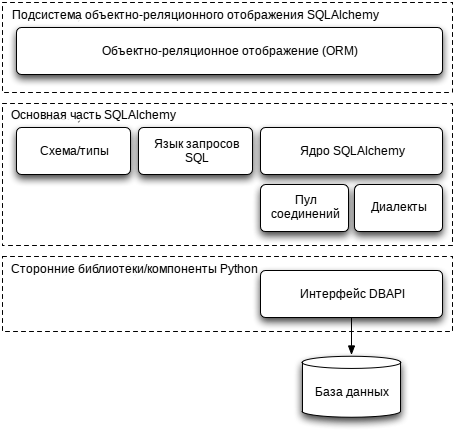
\includegraphics[height=\textheight]{media/sqlalchemy_layers_ru.png}
  \end{center}

\end{frame}

\begin{frame}{SQLAlchemy - Преимущества}

  \begin{itemize}

    \item \textbf{Безопасность}. Параметры запросов экранируются, что делает
      атаки типа внедрение SQL-кода маловероятными.
    \item \textbf{Производительность}. Повышается вероятность повторного
      использования запроса к серверу базы данных, что может позволить ему в
      некоторых случаях применить повторно план выполнения запроса.
    \item \textbf{Переносимость}. SQLAlchemy, при должном подходе, позволяет
      писать код на Python, совместимый с несколькими back-end СУБД.

  \end{itemize}

\end{frame}

\begin{frame}[fragile]{SQLAlchemy - Пример}

    \begin{lstlisting}[style=python]
    >>> from sqlalchemy import create_engine
    >>> engine = create_engine('sqlite:///:memory:')
    >>> engine.execute("select 'Hello, World!'").scalar()
    u'Hello, World!'
    \end{lstlisting}

\end{frame}

\begin{frame}[fragile]{SQLAlchemy - Пример}

  \url{https://bitbucket.org/zzzeek/pycon2013_student_package}

\end{frame}


\end{document}
